\section{模板 Stencil}
模板是流体动力学、热导、燃烧、天气预报、气候模拟和电磁学等应用领域中求解偏微分方程数值方法的基础。 
基于模板的算法处理的数据由具有物理意义的离散量组成,例如质量、速度、力、加速度、温度、电场和能量,
它们之间的关系由微分方程控制。 模板的常见用途是根据输入变量值范围内的函数值来近似函数的导数值。 
模板与卷积非常相似,因为模板和卷积都根据同一位置的元素的当前值以及另一个多维数组中邻域中的元素的当前值
来计算多维数组的元素的新值。 因此模板还需要处理光环单元和鬼单元。 与卷积不同,模板计算用于迭代求解感兴趣域内连续、可微函数的值。 
用于模板邻域中的元素的数据元素和权重系数由正在求解的微分方程控制。 某些模板图案适合不适用于卷积的优化。 
在初始条件通过域迭代传播的求解器中,输出值的计算可能具有依赖性,并且需要根据某些排序约束来执行。 
此外,由于解决微分问题时对数值精度的要求,模板处理的数据往往是高精度的浮点数据,这会消耗更多的片上内存用于平铺技术。 
由于这些差异,模板往往会引发与卷积不同的优化。

\subsection{背景}
\begin{figure}[H]
	\centering
	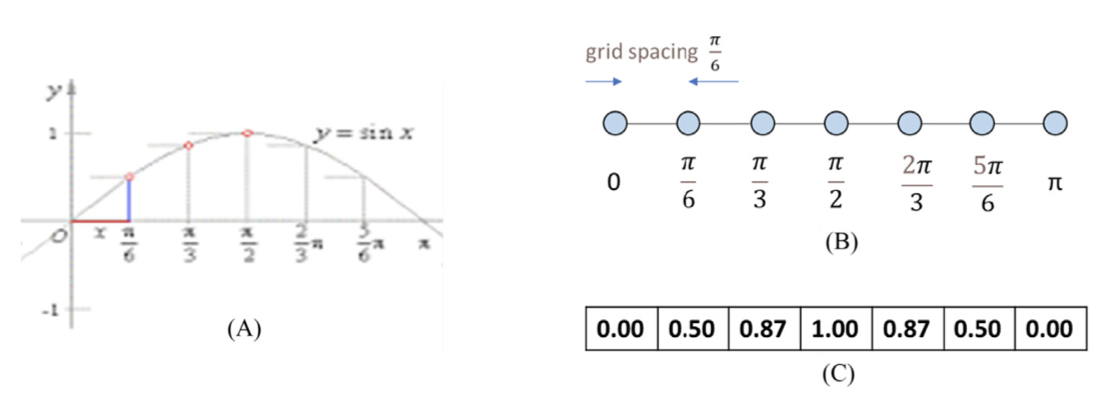
\includegraphics[width=0.9\textwidth]{figs/F8.1.png}
	\caption{\textit{(A) 正弦作为 $0 \leq x \leq \pi$ 的连续、可微函数。 
	(B) 设计具有网格点之间恒定间距($\frac{\pi}{6}$)的规则网格进行离散化。(C) $0 \leq x \leq\pi$ 的正弦函数的离散表示。}}
\end{figure}

使用计算机对函数、模型、变量和方程进行数值评估和求解的第一步是将它们转换为离散表示。 
例如,图 8.1A 显示了 $0 \leq x \leq \pi$ 的正弦函数 $y = \sin(x)$。 
图 8.1B 显示了一维 (1D) 规则(结构化)网格的设计,其七个网格点对应于具有恒定间距($\frac{\pi}{6}$ 间隔)的 x 值。
一般来说,结构化网格覆盖 n 维欧几里得 具有相同平行四面体的空间(例如,一维的线段、二维的矩形、三维的砖块)。
正如我们稍后将看到的,使用结构化网格,变量的导数可以方便地表示为有限差分。因此,主要使用结构化网格 在有限差分方法中。
非结构化网格更加复杂,用于有限元和有限体积方法。为简单起见,我们将仅使用规则网格,因此在本书中使用有限差分方法。

图 8.1C 显示了最终的离散表示,其中正弦函数用七个网格点处的值表示。 在这种情况下,表示形式存储在一维数组 F 中。
请注意,x 值隐式假定为 i6 π ,其中 i 是数组元素的索引。 例如,元素 F[2] 对应的 x 值为 0.87,即 26 π 的正弦值。

在离散表示中,需要使用线性或样条等插值技术来导出不对应于任何网格点的 x 值的函数近似值。 
表示的保真度或这些近似插值技术的函数值的精确度取决于网格点之间的间距:间距越小,近似值越精确。 
通过减小间距,可以提高表示的准确性,但代价是需要更多的存储空间,并且正如我们将看到的,在求解偏微分方程时需要更多的计算。

离散表示的保真度还取决于所使用的数字的精度。 由于我们正在逼近连续函数,因此浮点数通常用于网格点值。 
目前主流 CPU 和 GPU 支持双精度(64 位)、单精度(32 位)和半精度(16 位)表示。 
在这三者中,双精度数字在离散表示中提供了最好的精度和最高的保真度。 
然而,现代 CPU 和 GPU 对于单精度和半精度算术通常具有更高的算术计算吞吐量。 
此外,由于双精度数由更多位组成,因此读写双精度数会消耗更多内存带宽。 存储这些双精度数字也需要内存容量。 
这可能对需要将大量网格点值存储在片上存储器和寄存器中的平铺技术构成重大挑战。

让我们以更形式化的方式讨论模板的定义。 在数学中,模板是应用于结构化网格的每个点的权重的几何图案。 
该模式指定如何使用数值近似例程从相邻点的值导出感兴趣的网格点的值。 
例如,模板可以指定如何通过使用该点处的函数值与其邻居处的函数值之间的有限差来近似该点处函数的导数值。 
由于偏微分方程表达了函数、变量及其导数之间的关系,因此模板为指定有限差分方法如何数值计算偏微分方程的解提供了方便的基础。

例如,假设我们将 $f(x)$ 离散化为一维网格数组 F,并且我们想要计算 $f(x)$ 的离散化导数,$f'(x)$。 
我们可以使用经典的有限差分近似来计算一阶导数:
$$
f^{\prime}(x)=\frac{f(x+h)-f(x-h)}{2 h}+O\left(h^{2}\right)
$$

也就是说,函数在点x处的导数可以通过两个相邻点处的函数值的差除以这些相邻点的x值的差来近似。 
h 值是网格中相邻点之间的间距。 误差用 $O(h^2)$ 项表示; 这意味着误差与 h 的平方成正比。 
显然,h 值越小,近似效果越好。 在图 8.1 的示例中,h 值为 $\frac{\pi}{6}$ 或 0.52。 
该值不足以小到使近似误差可以忽略不计,但应该能够产生相当接近的近似值。

由于网格间距为 h,因此当前估计的 $f(x - h)$、$f(x)$ 和 $f(x + h)$ 值分别位于 $F[i - 1]$、$F[i]$ 和 $F[i + 1]$ 中,
其中 $x=i*h$。 因此我们可以将每个网格点的f(x)的导数值计算成输出数组FD:
$$
F D[i]=\frac{F[i+1]-F[i-1]}{2 * h}
$$

对于所有的网格点。 这个表达式可以重写为
$$
F D[i]=\frac{-1}{2 * h} * F[i-1]+\frac{1}{2 * h} * F[i+1]
$$

\begin{figure}[H]
	\centering
	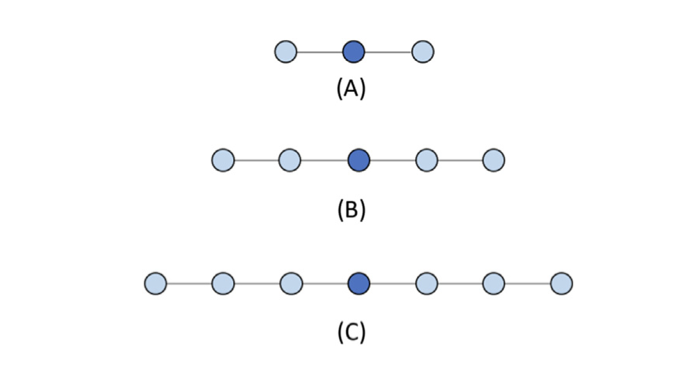
\includegraphics[width=0.9\textwidth]{figs/F8.2.png}
	\caption{\textit{一维模板示例。 (A) 三点(1 阶)模板。 (B) 五点(2 阶)模板。 (C) 七点(顺序 3)模板。}}
\end{figure}

即网格点估计函数导数值的计算涉及到当前网格点 $[i - 1, i, i + 1]$ 的估计函数值,
系数为 $\left[\frac{-1}{2 h}, 0, \frac{1}{2 h}\right]$,
定义了一个一维三-点模板,如图8.2A所示。 如果我们在网格点处近似更高的导数值,我们将需要使用高阶有限差分。 
例如,如果微分方程最多包含 f(x) 的二阶导数,
我们将使用包含 $[\mathrm{i}-2, \mathrm{i}-1, \mathrm{i}, \mathrm{i}+1, \mathrm{i}+2]$ 的模板,
这是一个一维五-点模板,如图8.2B所示。 一般来说,如果方程涉及到 n 阶导数,则模板将涉及中心网格点每一侧的 n 个网格点。 
图 8.2C 显示了 1D 七点模板。 中心点每侧的网格点数量称为模板的阶数,因为它反映了被逼近的导数的阶数。 
根据这个定义,图 8.3 中的模板分别为 1、2 和 3 阶。

\begin{figure}[H]
	\centering
	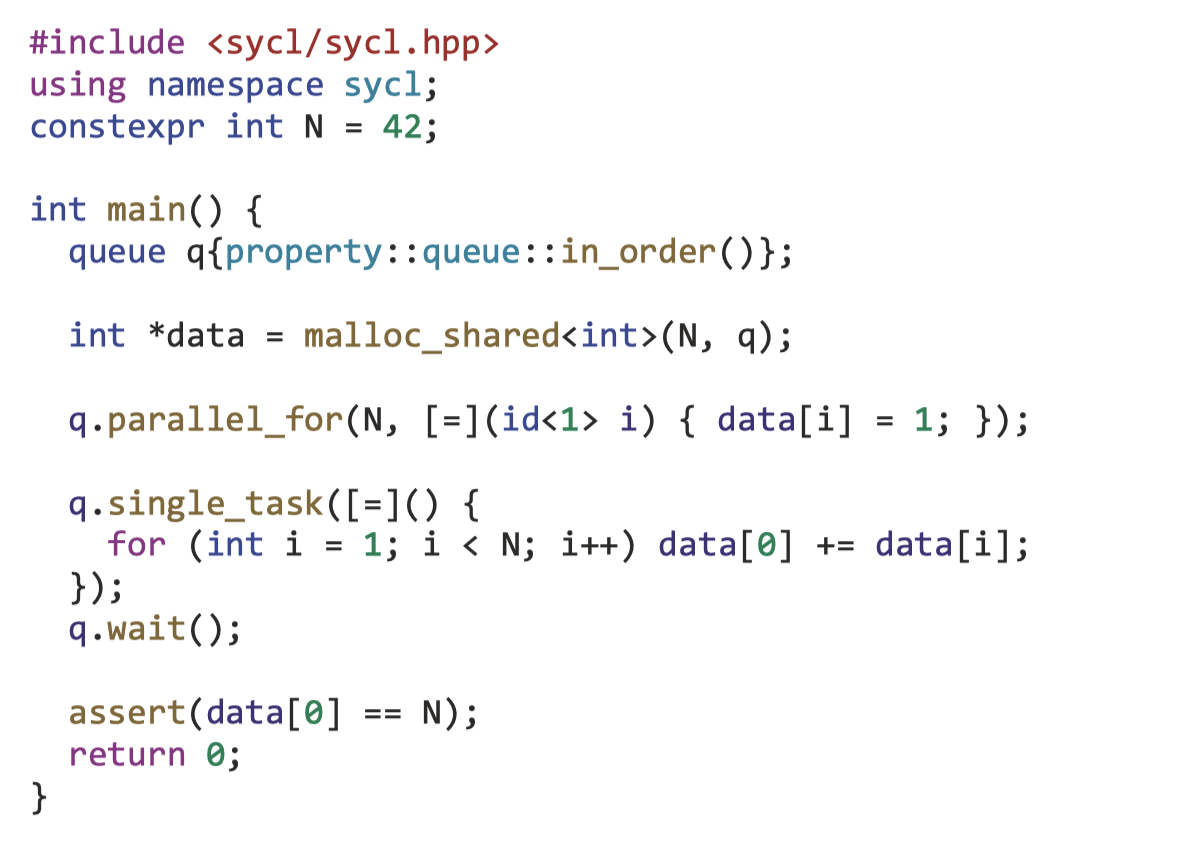
\includegraphics[width=0.9\textwidth]{figs/F8.3.png}
	\caption{\textit{(A) 二维五点模板(1阶)。 (B) 二维九点模板(2阶)。 (C) 三维七点模板(1阶)。 (D) 三维 13 点模板(2阶)。}}
\end{figure}

显然,求解两个变量的偏微分方程需要将函数值离散化为二维 (2D) 网格,我们将使用 2D 模板来计算近似偏导数。 
如果偏微分方程只涉及其中一个变量的偏导数,
例如 $\frac{\partial f(x, y)}{\partial x}, \frac{\partial f(x, y)}{\partial y}$ ,
但不是 $\frac{\partial f(x, y)}{\partial x \partial y}$ ,
我们可以使用所选网格点都沿 x 轴和 y 轴的 2D 模板。 例如,对于仅涉及 x 的一阶导数和 y 的一阶导数的偏微分方程,
我们可以使用包含沿 x 轴和 y 轴在中心点两侧各有两个网格点的 2D 模板,结果为 图 8.3A 中的 2D 五点模板。 
如果方程仅涉及 x 或 y 的二阶导数,我们将使用二维九点模板,如图 8.3B 所示。

\begin{figure}[H]
	\centering
	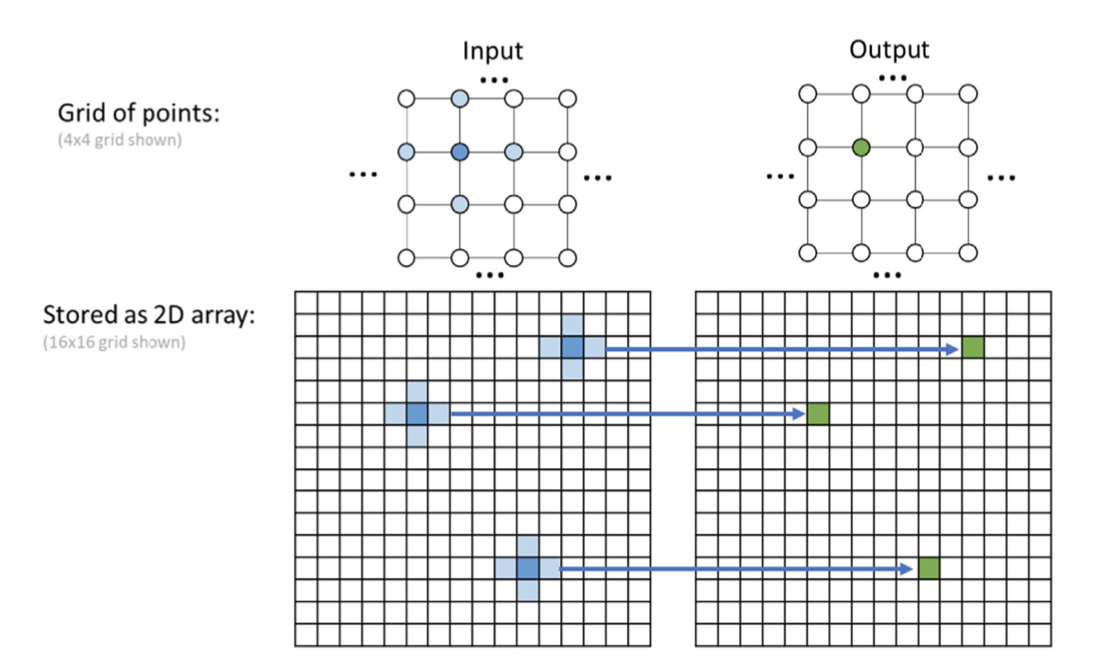
\includegraphics[width=0.9\textwidth]{figs/F8.4.png}
	\caption{\textit{二维网格示例和用于计算网格点处的近似导数值的五点(1 阶)模板。}}
\end{figure}

图 8.4 总结了离散化、数值网格以及网格点上模板的应用的概念。 函数被离散化为其网格点值,并存储在多维数组中。 
在图 8.4 中,两个变量的函数被离散化为 2D 网格,并存储为 2D 数组。 
图 8.4 中使用的模板是 2D 的,用于根据相邻网格点和网格点本身的函数值计算每个网格点的近似导数值(输出)。 
在本章中,我们将重点关注将模板应用于所有相关输入网格点以在所有网格点生成输出值的计算模式,这将被称为模板扫描。

\subsection{并行模板:基础算法}
\begin{figure}[H]
	\centering
	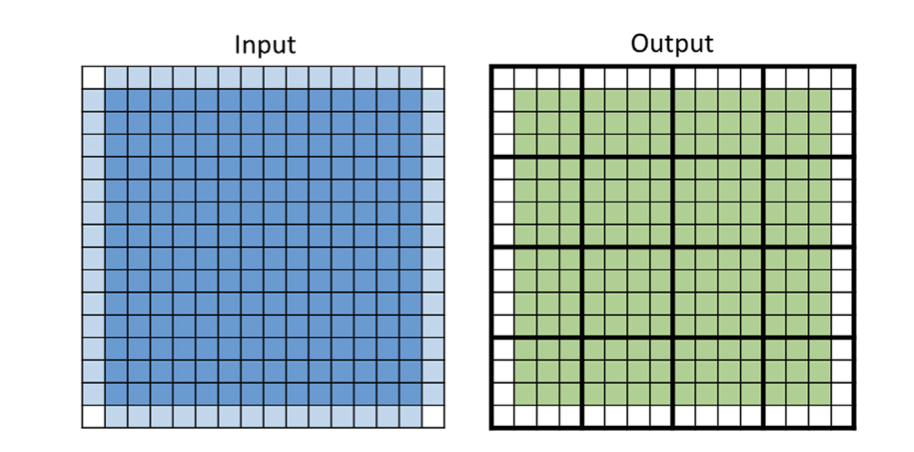
\includegraphics[width=0.9\textwidth]{figs/F8.5.png}
	\caption{\textit{简化边界条件。 边界单元包含不会从一次迭代到下一次迭代更新的边界条件。 
	因此,在每次模板扫描期间仅需要计算内部输出网格点。}}
\end{figure}

我们将首先介绍模板扫描的基本内核。 为简单起见,我们假设在模板扫描内生成输出网格点值时,输出网格点之间不存在依赖性。 
我们进一步假设边界上的网格点值存储边界条件并且不会从输入到输出改变,如图8.5所示。 
也就是说,将计算输出网格中的阴影内部区域,而未阴影的边界单元将保持与输入值相同。 
这是一个合理的假设,因为模板主要用于求解具有边界条件的微分方程。

\begin{figure}[H]
	\centering
	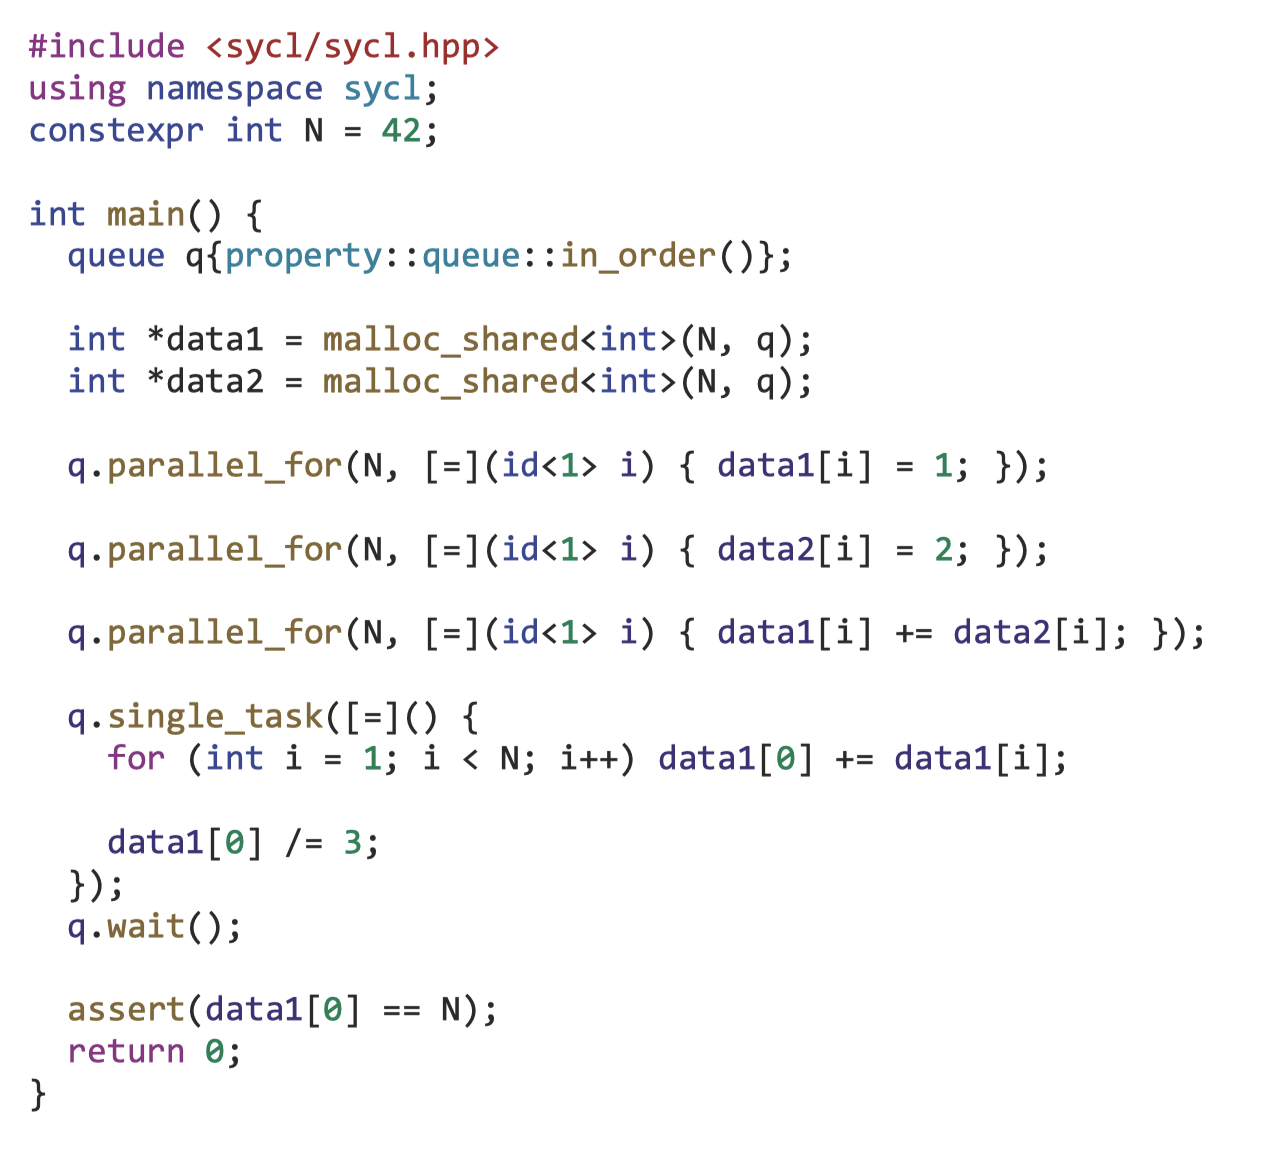
\includegraphics[width=0.9\textwidth]{figs/F8.6.png}
	\caption{\textit{基本的模板扫描内核。}}
\end{figure}

图 8.6 显示了执行模板扫描的基本内核。 该内核假设每个线程块负责计算输出网格值的图块,并且每个线程都被分配给一个输出网格点。 
图 8.5 显示了输出网格的 2D 平铺示例,其中每个线程块负责 $4 \times 4$ 输出平铺。 
然而,由于大多数实际应用程序求解三维 (3D) 微分方程,因此图 8.6 中的内核假设有一个 3D 网格和一个 3D 七点模板,
如图 8.3C 中所示。 线程到网格点的分配是通过熟悉的线性表达式完成的,
涉及 blockIdx、blockDim 和 threadIdx 的 x、y 和 z 字段(第 02-04 行)。 将每个线程分配给 3D 网格点后,
该网格点和所有相邻网格点的输入值将乘以不同的系数(第 06-12 行上的 c0 到 c6)并相加。 
正如我们在背景部分中所解释的,这些系数的值取决于正在求解的微分方程。

现在让我们计算图 8.6 中内核的浮点与全局内存访问比率。 每个线程执行 13 次浮点运算(七次乘法和六次加法)并加载七个输入值,
每个值 4 字节。 因此,该内核的浮点与全局内存访问比率为 $13/(7 * 4) = 0.46 OP/B$(每字节操作数)。 
正如我们在第 5 章“内存架构和数据局部性”中讨论的那样,该比率需要大得多,内核的性能才能合理地接近算术计算资源支持的水平。 
我们需要使用第 7 章“卷积”中讨论的平铺技术来提高浮点与全局内存访问的比率。

\subsection{用于模板扫描的共享内存平铺}
正如我们在第 5 章“内存架构和数据局部性”中看到的,通过共享内存平铺可以显着提高浮点操作与全局内存访问操作的比率。 
正如读者可能怀疑的那样,模板的共享内存平铺设计几乎与卷积的设计相同。 然而,存在一些微妙但重要的差异。

\begin{figure}[H]
	\centering
	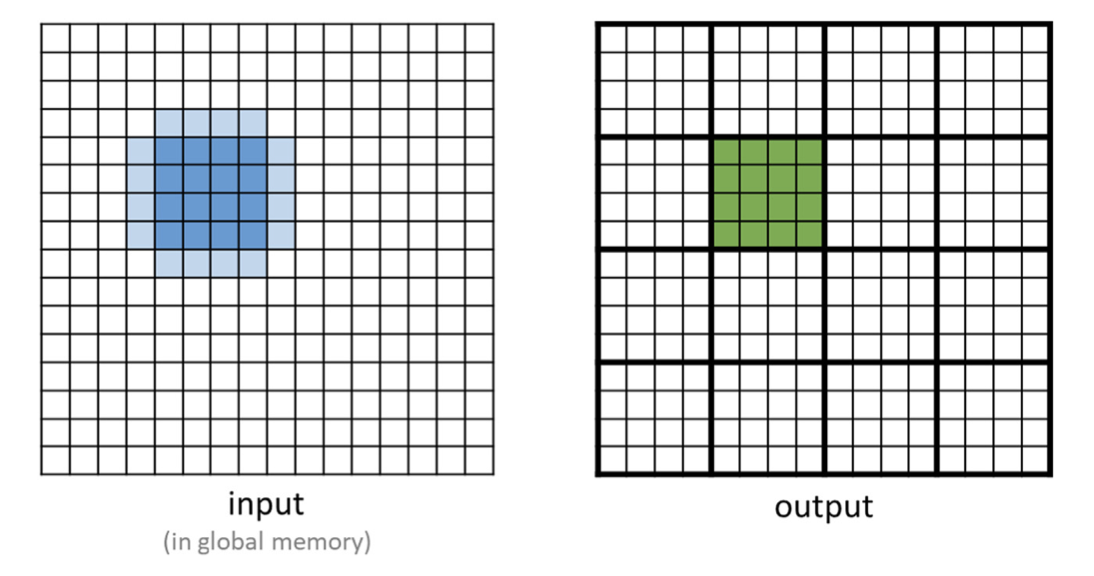
\includegraphics[width=0.9\textwidth]{figs/F8.7.png}
	\caption{\textit{二维五点模板的输入和输出图块。}}
\end{figure}

图 8.7 显示了应用于小网格示例的 2D 五点模板的输入和输出图块。 
与图 7.11 的快速比较显示了卷积和模板扫描之间的微小差异:五点模板的输入图块不包括角网格点。 
当我们在本章后面探讨寄存器平铺时,这个属性将变得很重要。 出于共享内存平铺的目的,
我们可以预期 2D 五点模板中的输入数据重用将显着低于 $3 \times 3$ 卷积中的输入数据重用。 
正如我们在第 7 章“卷积”中讨论的那样,2D $3 \times 3$ 卷积的算术与全局内存访问比率的上限是 4.5 OP/B。 
然而,对于 2D 五点模板,该比率的上限仅为 2.5 OP/B。 这是因为与 $3 \times 3$ 卷积中的 9 个输入像素值相比,
每个输出网格点值仅使用 5 个输入网格值。

当模板的维数和阶数增加时,这种差异甚至更加明显。 
例如,如果我们将 2D 模板的阶数从 1(每侧一个网格点,五点模板)增加到 2(每侧两个网格点,九点模板),
则比率的上限为 4.5 OP/B,与其对应的 2D $5 \times 5$ 卷积的 12.5 OP/B 相比。 
当 2D 模板的阶数增加到 3(每侧 3 个网格点,13 点模板)时,这种差异更加明显。 
该比率的上限为 6.5 OP/B,而其对应的 2D $7 \times 7$ 卷积的上限为 24.5 OP/B。

当我们进入 3D 时,模板扫描和卷积的算术与全局内存访问比率的上限之间的差异更加明显。 
例如,3D 三阶模板(每侧 3 个点,19 点模板)的上限为 9.5 OP/B,
而其对应的 3D $7 \times 7 \times 7$ 卷积的上限为 171.5 OP/B。 
也就是说,将输入网格点值加载到共享内存中进行模板扫描的好处可能明显低于卷积的好处,特别是对于 3D,这是模板的主要用例。 
正如我们将在本章后面看到的,这种微小但显着的差异激发了在第三维中使用线程粗化和寄存器平铺。

\begin{figure}[H]
	\centering
	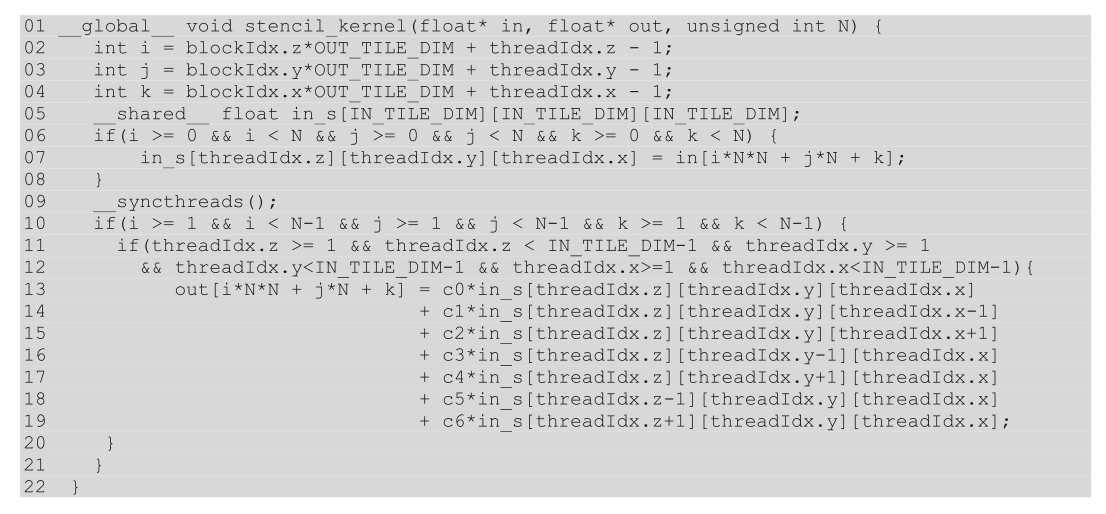
\includegraphics[width=0.9\textwidth]{figs/F8.8.png}
	\caption{\textit{具有共享内存平铺的 3D 七点模板扫描内核。}}
\end{figure}

由于加载输入图块进行卷积的所有策略都直接应用于模板扫描,因此我们在图 8.8 中呈现了一个类似于图 7.12 中的卷积内核的内核,
其中块的大小与输入图块相同,并且一些线程被关闭 在计算输出网格点值时。 
该内核是根据图 8.6 中的基本模板扫描内核改编的,因此我们将只关注改编期间所做的更改。 
与平铺卷积内核一样,平铺模板扫描内核首先计算用于每个线程的输入补丁的起始 x、y 和 z 坐标。 
每个表达式中减去的值 1 是因为内核假定一个 3D 七点模板,每一侧都有一个网格点(第 02-04 行)。 
一般来说,减去的值应该是模板的阶数。

内核在共享内存中分配一个 in\_s 数组来保存每个块的输入图块(第 05 行)。 每个线程加载一个输入元素。 
与平铺卷积核一样,每个线程加载包含模板网格点模式的立方输入补丁的起始元素。 
由于第 02-04 行中的减法,某些线程可能会尝试加载网格的幽灵单元。 
条件 $i >=0, j>= 0$, 以及 $k >= 0$(第 06 行)防止这些越界访问。 
由于块比输出图块大,因此块的 x、y 和 z 维度末尾的某些线程也可能尝试访问网格每个维度上限之外的幻影单元 大批。 
条件 $I < N, j < N$ 和 $k < N$ (第 6 行)可防止这些越界访问。 
线程块中的所有线程协作将输入图块加载到共享内存中(第 07 行),并使用屏障同步等待,
直到所有输入图块网格点都位于共享内存中(第 09 行)。

每个块在第 10-21 行计算其输出图块。 第 10 行中的条件反映了简化的假设,即输入网格和输出的边界点都保存初始条件值,
并且不需要由内核从迭代到迭代进行计算。 因此,输出网格点落在这些边界位置上的线程将被关闭。 
请注意,边界网格点在网格表面形成一层。

第 12-13 行中的条件关闭只是为了加载输入图块网格点而启动的额外线程。 
这些条件允许那些 i、j 和 k 索引值落在输出图块内的线程计算由这些索引选择的输出网格点。 
最后,每个活动线程使用七点模板指定的输入网格点计算其输出网格点值。

我们可以通过计算该内核实现的算术与全局内存访问比率来评估共享内存平铺的有效性。 
回想一下,原始的模板扫描内核实现了 0.46 OP/B 的比率。 
对于共享内存平铺内核,我们假设每个输入平铺都是一个每个维度都有 T 个网格点的立方体,
并且每个输出平铺在每个维度都有 $T - 2$ 个网格点。 
因此每个块有 $(T - 2)^3$ 个活动线程计算输出网格点值,
每个活动线程执行 13 次浮点乘法或加法运算,总共 $13 \times (T - 2)^3$ 次浮点算术运算 。 
此外,每个块通过执行各自为4字节的 $T^3$ 加载来加载输入图块。 因此,平铺内核的浮点与全局内存访问比率可以计算如下:
$$
\frac{13 *(T-2)^{3}}{4 * T^{3}}=\frac{13}{4} *\left(1-\frac{2}{T}\right)^{3} \quad O P / B
$$

也就是说,$T$ 值越大,输入的网格点值被重用的次数就越多。 随着 $T$ 渐近增加,该比率的上限为 $13/4 = 3.25$ OP/B。

不幸的是,当前硬件上块大小的 1024 限制使得很难拥有大的 $T$ 值。 
$T$ 的实际限制是 8,因为 $8 \times 8 \times 8$ 线程块总共有 512 个线程。 
此外,用于输入图块的共享存储器的量与 $T^3$ 成比例。 
因此,较大的 $T$ 会显着增加共享内存的消耗。 这些硬件限制迫使我们对平铺模板内核使用较小的平铺尺寸。 
相反,卷积通常用于处理 2D 图像,其中可以使用较大的图块尺寸($T$ 值),例如 $32 \times 32$。

硬件对 T 值施加的小限制有两个主要缺点。 第一个缺点是它限制了重用率,从而限制了计算与内存访问的比率。 
对于 T = 8,七点模板的比率仅为 1.37 OP/B,远小于 3.25 OP/B 的上限。 由于光环开销,重用率随着 T 值的减小而减小。 
正如我们在第 7 章“卷积”中讨论的那样,光环元素的重用率低于非光环元素。 
随着输入图块中光环元素部分的增加,数据重用率和浮点与全局存储器访问率都会降低。 
例如,对于半径为 1 的卷积滤波器,$32 \times 32$ 2D 输入图块具有 1024 个输入元素。 
相应的输出图块有 $30 \times 30 = 900$ 个元素,这意味着 $1024 - 900 = 124$ 个输入元素是光环元素。 
输入图块中光环元素的比例约为 12\%。 相反,对于 1 阶 3D 模板,$8 \times 8 \times 8$ 3D 输入图块具有 512 个元素。 
相应的输出图块具有 $6 \times 6 \times 6 = 216$ 个元素,这意味着 $512 - 216 = 296$ 个输入元素是光环元素。 
输入图块中光环元素的比例约为 58%!

小图块大小的第二个缺点是它会对内存合并产生不利影响。 
对于 $8 \times 8 \times 8$ 图块,由 32 个线程组成的每个扭曲将负责加载图块的四个不同行,每个行有八个输入值。 
因此,在同一条加载指令上,warp 的线程将访问全局内存中的至少四个远程位置。 这些访问无法合并,并且不会充分利用 DRAM 带宽。 
因此,T 需要是一个更大的值,以便重用级别更接近 3.25 OP/B 并能够充分利用 DRAM 带宽。 
对更大 T 的需求激发了我们将在下一节中介绍的方法。

\subsection{线程粗化}
正如我们在上一节中提到的,模板通常应用于 3D 网格,并且模板图案的稀疏性质使得模板扫描成为共享内存平铺的利润比卷积更低的目标。 
本节介绍如何使用线程粗化来克服块大小限制,方法是将每个线程完成的工作从计算一个网格点值粗化为一列网格点值,如图 8.9 所示。 
回想一下第 6.3 节,通过线程粗化,程序员将并行工作单元部分序列化到每个线程中,并降低了并行性所付出的代价。 
在这种情况下,为并行性付出的代价是由于每个块加载光环元素而导致的低数据重用。

\begin{figure}[H]
	\centering
	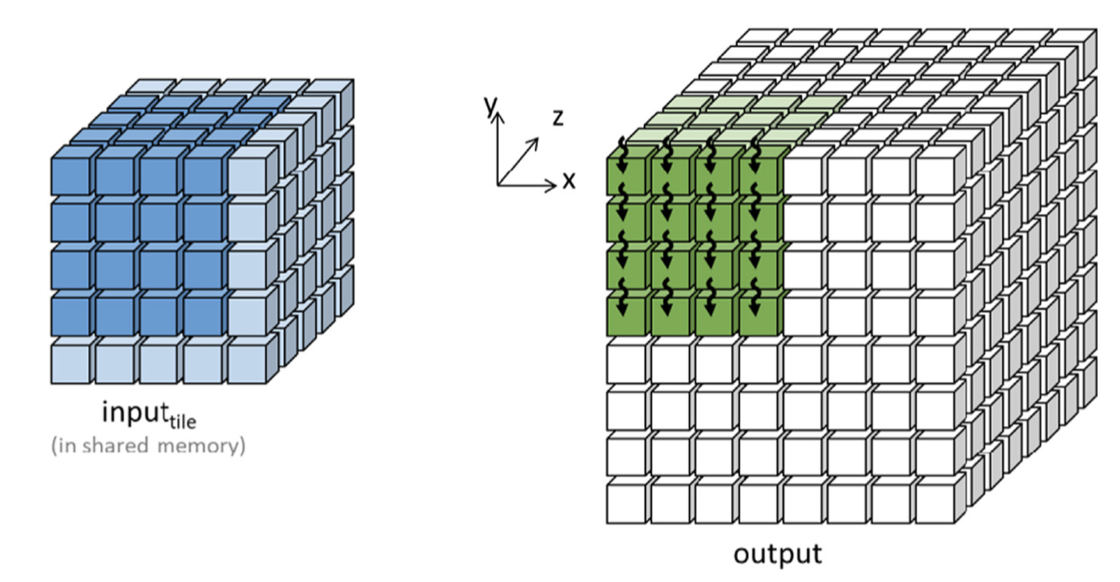
\includegraphics[width=0.9\textwidth]{figs/F8.9.png}
	\caption{\textit{z 方向上的线程粗化,用于 3D 七点模板扫描。}}
\end{figure}

在图 8.9 中,我们假设每个输入图块由 $T^3 = 6^3 = 216$ 个网格点组成。 
请注意,为了使输入图块的内部可见,我们剥离了图块的前层、左层和顶层。 
我们还假设每个输出图块由 $(T-2)^3 = 4^3 = 64$ 个网格点组成。 图中的 x、y 和 z 方向与输入和输出的坐标系一起显示。 
输入图块的每个 x-y 平面由 $6^2 = 36$ 个网格点组成,输出图块的每个 x-y 平面由 $4^2 = 16$ 个网格点组成。 
分配用于处理该图块的线程块由与输入图块的一个 x-y 平面相同数量的线程组成(即 $6 \times 6$)。 
在图中,我们仅显示了在计算输出图块值时处于活动状态的线程块的内部线程(即 $4 \times 4$)。

\begin{figure}[H]
	\centering
	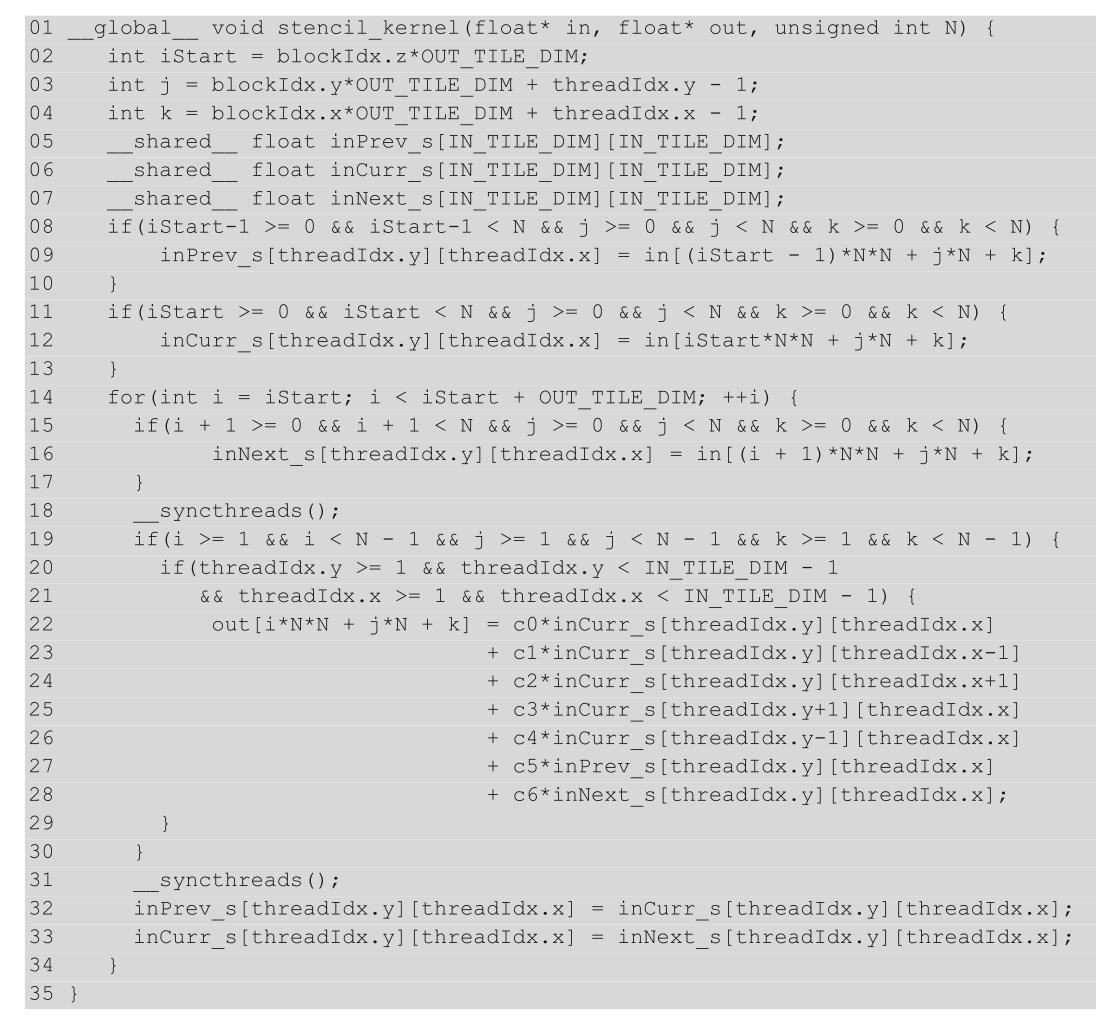
\includegraphics[width=0.9\textwidth]{figs/F8.10.png}
	\caption{\textit{在 z 方向上进行线程粗化的内核,用于 3D 七点模板扫描。}}
\end{figure}

图 8.10 显示了在 z 方向上进行线程粗化的内核,用于 3D 七点模板扫描。 
这个想法是让线程块在 z 方向(进入图中)迭代,在每次迭代期间计算输出图块的一个 x-y 平面中的网格点的值。 
内核首先将每个线程分配给输出的 x-y 平面中的一个网格点(第 03-04 行)。 注意,i是每个线程计算的输出瓦片网格点的z索引。 
在每次迭代期间,块中的所有线程都将处理输出图块的 x-y 平面; 因此它们都将计算 z 索引相同的输出网格点。

最初,每个块需要将三个输入图块平面加载到共享内存中,
这些输入图块平面包含计算图 8.9 中最接近读取器(用线程标记)的输出图块平面的值所需的所有点。 
这是通过让块中的所有线程将第一层(第 08-10 行)加载到共享内存数组 inPrev\_s 中,
并将第二层(第 11-13 行)加载到共享内存数组 inCurr\_s 中来完成的。 
对于第一层,inPrev\_s 是从输入图块的前层加载的,该图块已被剥离以查看内部层。

在第一次迭代期间,块中的所有线程协作将当前输出图块层所需的第三层加载到共享内存数组 inNext\_s 中(第 15-17 行)。 
然后,所有线程都在屏障上等待(第 18 行),直到所有线程都完成加载输入图块层。 
第 19-21 行中的条件与图 8.8 中共享内存内核中的条件具有相同的用途。

然后,每个线程使用 inCurr\_s 中存储的四个 x-y 邻居、inPrev\_s 中的 z 邻居
以及 inNext\_s 中的 z 邻居计算其在当前输出图块平面中的输出网格点值。 
然后,块中的所有线程在屏障处等待,以确保每个人都完成计算,然后再移动到下一个输出图块平面。 
一旦脱离屏障,所有线程协作将 inCurr\_s 的内容移动到 inPrev\_s 并将 inNext\_s 的内容移动到 inCurr\_s。 
这是因为当线程沿 z 方向移动一个输出平面时,输入图块平面所扮演的角色会发生变化。 
因此,到每次迭代结束时,该块具有计算下一次迭代的输出瓦片平面所需的三个输入瓦片平面中的两个。 
然后,所有线程都进入下一次迭代,并加载迭代输出平面所需的输入图块的第三个平面。 
为第二个输出图块平面的计算做准备的更新后的 inPrev\_s、inCurr\_s 和 inNext\_s 映射如图 8.11 所示。

\begin{figure}[H]
	\centering
	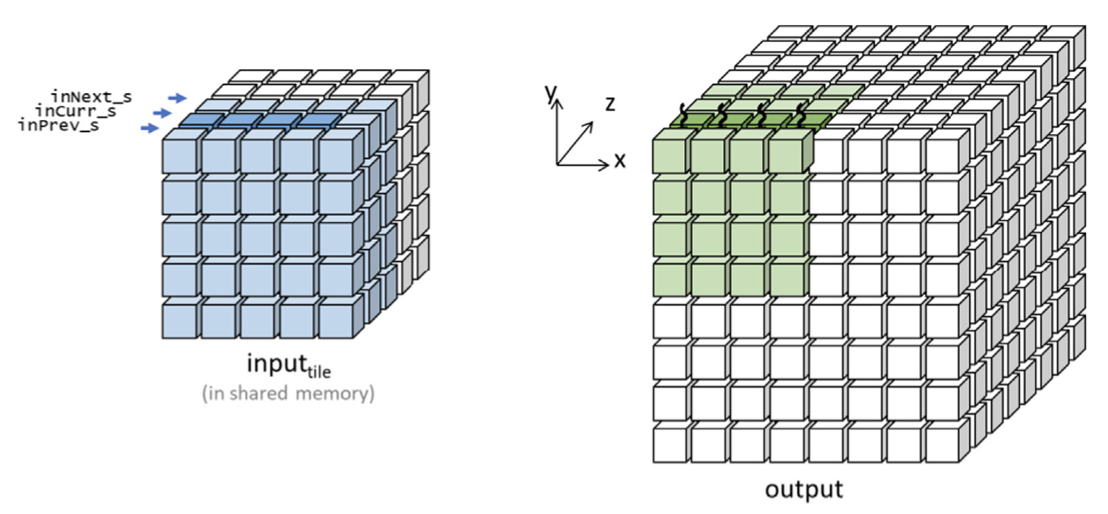
\includegraphics[width=0.9\textwidth]{figs/F8.11.png}
	\caption{\textit{第一次迭代后共享内存数组到输入图块的映射。}}
\end{figure}

线程粗化内核的优点在于,它在不增加线程数量的情况下增加了图块大小,并且不需要输入图块的所有平面都存在于共享内存中。 
线程块大小现在仅为 $T^2$ 而不是 $T^3$ ,因此我们可以使用更大的 T 值,例如 32,这将导致块大小为 1024 个线程。 
有了这个 $T$ 值,我们可以预期浮点运算与全局内存访问的比率将为 
$\frac{13}{4} *\left(1-\frac{2}{32}\right)^{3}=2.68 \mathrm{OP} / \mathrm{B}$,
这比 1.37 的 OP/ B 比率有显着改善。 原始共享内存平铺内核,更接近 3.25 OP/B 上限。 
此外,在任何时间点,只有三层输入图块需要位于共享内存中。 共享内存容量要求现在是 $3T^2$ 个元素,而不是 $T^3$ 个元素。 
对于 $T = 32$,共享内存消耗现在处于每块 $3 * 32^{2} * 4 \mathrm{~B}=12 \mathrm{~KB}$ 的合理水平。

\subsection{寄存器平铺}
一些模板图案的特殊特性可以带来新的优化机会。 
在这里,我们提出了一种优化,对于仅涉及中心点沿 x、y 和 z 方向的邻居的模板图案特别有效。 
图 8.3 中的所有模板都属于此描述。 图 8.10 中的 3D 七点模板扫描内核反映了这一特性。 
每个 inPrev\_s 和 inNext\_s 元素仅由一个线程用于计算具有相同 x-y 索引的输出图块网格点。 
只有 inCurr\_s 元素被多个线程访问并且真正需要位于共享内存中。 
inPrev\_s 和 inNext\_s 中的 z 邻居可以保留在单个用户线程的寄存器中。

\begin{figure}[H]
	\centering
	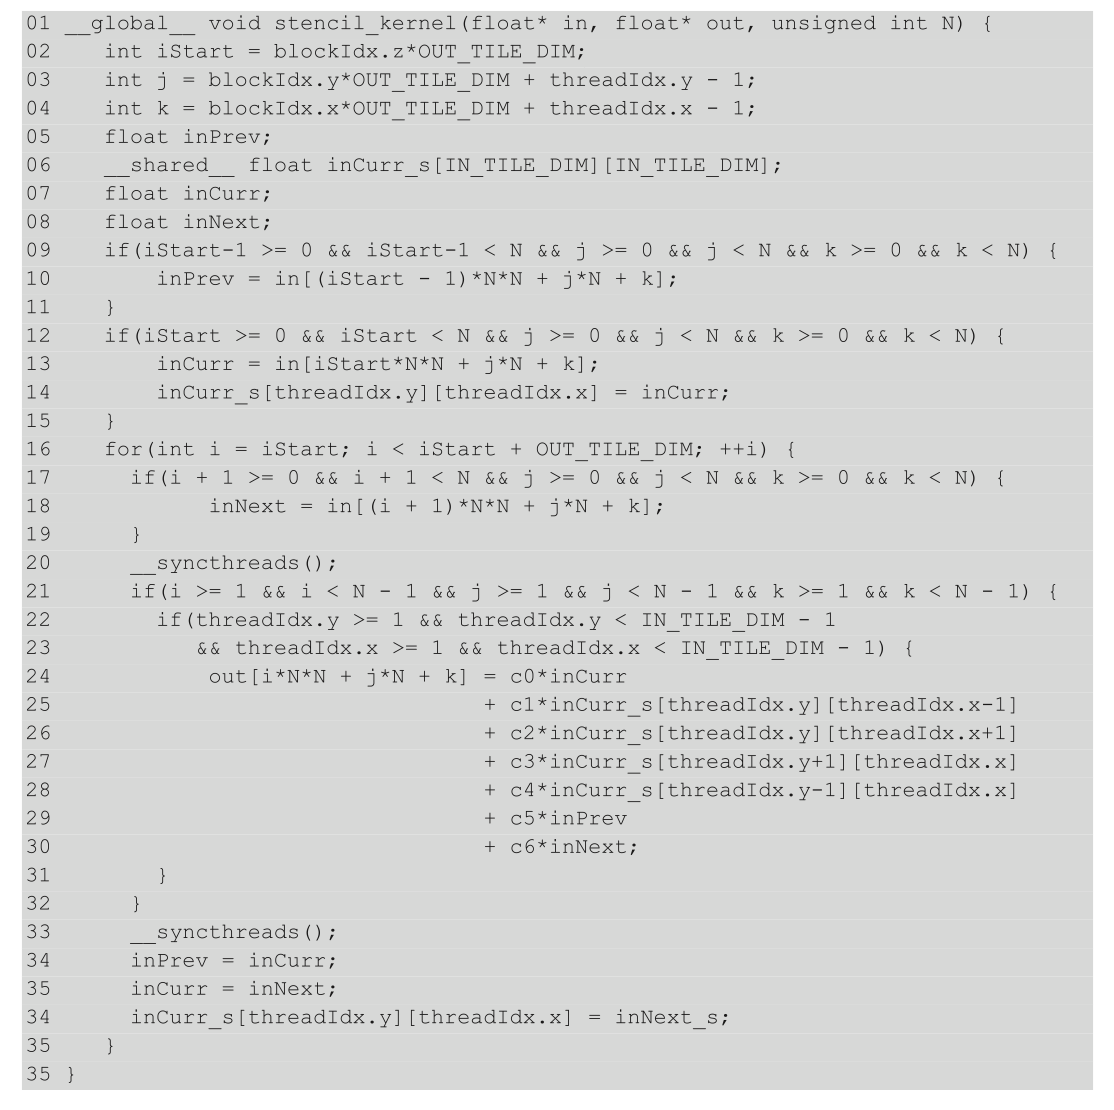
\includegraphics[width=0.9\textwidth]{figs/F8.12.png}
	\caption{\textit{内核在 z 方向上具有线程粗化和寄存器平铺功能,用于 3D 七点模板扫描。}}
\end{figure}

我们利用图 8.12 中的寄存器平铺内核的这一特性。 
该内核是在图 8.10 中的线程粗化内核的基础上构建的,并进行了一些简单但重要的修改。 我们将重点关注这些修改。 
首先,我们创建三个寄存器变量 inPrev、inCurr 和 inNext(第 05、07、08 行)。 
寄存器变量 inPrev 和 inNext 分别替换共享内存数组 inPrev\_s 和 inNext。 
相比之下,我们保留 inCurr\_s 以允许 x-y 相邻网格点值在线程之间共享。 
因此,该内核使用的共享内存量减少到图 8.12 中内核使用的共享内存量的三分之一。

先前和当前输入图块平面的初始加载(第 09-15 行)以及每次新迭代之前输入图块的下一个平面的加载(第 17-19 行)
都是以寄存器变量作为目标来执行的。 因此,输入图块的“活动部分”的三个平面被保存在跨同一块的线程的寄存器中。 
此外,内核始终在共享内存中维护输入图块的当前平面的副本(第 14 行和第 34 行)。 
也就是说,活动输入图块平面的 x-y 邻居始终可供需要访问这些邻居的所有线程使用。

图 8.10 和 8.12 中的内核都只将输入块的活动部分保留在片上存储器中。 
活动部分中的平面数量取决于模板的顺序,对于 3D 七点模板为 3。 
图 8.12 中的粗化和寄存器平铺内核比图 8.10 中的粗化内核有两个优点。 首先,许多对共享内存的读取和写入现在都转移到寄存器中。 
由于寄存器比共享内存具有显着更低的延迟和更高的带宽,因此我们期望代码运行得更快。 其次,每个块仅消耗共享内存的三分之一。 
当然,这是以每个线程多使用 3 个寄存器为代价的,或者每块多使用 3072 个寄存器(假设有 $32 \times 32$ 个块)。 
读者应该记住,对于高阶模板,寄存器的使用会变得更高。 如果寄存器的使用成为问题,则可以返回将一些平面存储在共享存储器中。 
这种情况代表了一种常见的权衡,通常需要在共享内存和寄存器使用之间进行权衡。

总体而言,数据重用现在分布在寄存器和共享内存中。 全局内存访问的数量没有改变。 
如果我们同时考虑寄存器和共享内存,则总体数据重用与仅将共享内存用于输入图块的线程粗化内核保持相同。 
因此,当我们将寄存器平铺添加到线程粗化时,不会对全局内存带宽的消耗产生影响。

请注意,我们之前已经见过将一块数据集中存储在块线程的寄存器中的想法。 
在第 3 章“多维网格和数据”和第 5 章“内存架构和数据局部性”中的矩阵乘法内核以及第 7 章“卷积”中的卷积内核中,
我们将每个线程计算的输出值存储在该线程的寄存器中。 因此,由块计算的输出图块被集中存储在该块的线程的寄存器中。 
因此,寄存器平铺并不是一种新的优化,而是我们之前应用过的优化。 
它在本章中变得更加明显,因为我们现在使用寄存器来存储部分输入图块:在整个计算过程中,
相同的图块有时存储在寄存器中,有时存储在共享内存中。

\subsection{总结}
在本章中,我们深入研究了模板扫描计算,这似乎只是与特殊滤波器模式的卷积。 
然而,由于模板来自求解微分方程时导数的离散化和数值逼近,因此它们具有激发和实现新优化的两个特征。 
第一次模板扫描通常在 3D 网格上完成,而卷积通常在 2D 图像或少量 2D 图像时间切片上完成。 
这使得两者之间的平铺考虑因素不同,并促进 3D 模板的线程粗化,以实现更大的输入平铺和更多的数据重用。 
其次,模板模式有时可以启用输入数据的寄存器平铺,以进一步提高数据访问吞吐量并减轻共享内存压力。